\documentclass{article}
\usepackage[utf8]{inputenc}
\usepackage[]{geometry}
\usepackage{amsmath}
\usepackage{graphicx}
\usepackage{caption}
\usepackage{amsmath}
\usepackage{amssymb}
\geometry{left=2.5cm, right=2.5cm, top=2.5cm, bottom=2.5cm}

\title{Modeling the Adaptability of Network Protocol}
\author{Translated by Lynn }
\date{September 27th, 2016}

\begin{document}

\maketitle

\section*{Abstract}
The adaptability of network protocol(ANP), which means whether the protocol can be deployed to the network
and used extensively after a period of evolution. Many protocols developed slowly or failed, although they
meet the requirements of design technically. We propose a new model which has two models to improve the ANP,
self-evolution model(SEM) before the protocols deployed to the network and user dynamic behavior evolution
model(UDBEM) after the protocols applied to the real network. SEM determines whether the new network protocol
can survive by simulating the evolution process of the protocol in the protocol stack. UDBEM counts the new
user's penetration by simulating the transformation process of new protocol users' states in logical network.
We propose a evaluation model on the basis of communication efficiency, then measure the ANP by calculating
the communication efficiency of the new protocols envolves to the final states through the model. We also
present some factors which affect the ANP and methods to improve the ANP by analyzing these factors. After
theoretic model simulation analysis, we draw some conclusions. The protocols at the waist of the hourglass
appear to have less survival, while the lower and higher layers tend to live longer and easier. Increasing
the utility, the external utility of the protocol and the efficiency of the converters appropriately play
important roles in improving the ANP. The network protocol adaptability evolution model we proposed can be
applied to assess the ANP.

\setlength{\parskip}{0.5\baselineskip}
\par\noindent \textbf {Key Words:}
Adaptability, Network Protocol, Communication Efficiency, Penetration

\section{Introduction}
The Internet community has specified a large number of protocols to date, although they were developed, these
protocols have achieved varying degrees of success. Two major dimensions on which a protocol can be evaluated
are scale and purpose. Purpose can be explained whether the protocol could meet the design goals, which belongs
to technical areas. Scale relates to the protocols are deployed at last, whether the numbers of users expected.
Lots of protocols were not deployed extensively. For example, IPv6 caused great concern since 1996, its deployment
and usage is not optimistic at the moment compared to IPv4[4]. Most research on IPv6 is focused on technical
research, such as, IP address allocation, dual stack coexistence, new network protocol and so on, which make
it dose not get enough attention about how to deploy and operate. That's why IPv6 develops so slowly although
we make lots of progress[5]. This shows the research and development about protocol is not just a technical
problem, but the benefits, deployment expense, switch costs are important factors about whether the protocols
can be accepted by users after the protocols are applied to the network[7][8]. The degree of users's acceptance
of the protocols called "adaptability" after they are applied to the network for a period. So not only the
features and performance should be focused but the adaptability when we develop the protocol. Research on the
ANP, enabling developers to focus on technology to improve performance while designing the protocol, follow
the protocol-related technology that focus on how to improve the adaptability of the protocol, increasing the
degree of users's acceptance. That makes different for lowering the costs and reducing the blindness of protocol
development. The emerging of various theories and methods lay a foundation for the ANP which makes the ANP a very
popular research at home and abroad. However, the research of TANP is never easy, because the developers did not
take economic, environment factors into consideration even based on false assumptions. Besides, common agreement
has not been reached about evaluate the ANP home and abroad, that's the problem to be solved.

\section{Problem Analysis}
The methods focused on the ANP research has two categories which is intuitive methods of measurement and modeling
analysis. Traditional studies suggest that there are five factors can affect the deployment of a new protocol,
they are relative advantage, compatibility, complexity, workability and observability. They study the effects of
economic factors, external network properties on the deployment of protocol from economic perspective by visiting
equipment manufacturers, application providers, ISP and users then evaluate the adaptability of IPv6[10].
Colitti.L et al evaluate the adaptability of IPv6 as a user. When users post HTTP requests, they can choose post
the data to the sever by IPv4 or by dual-stack. They apply this method to Google then count and analyze the post
data over past year, the result shows a small-scale IPv6 deployment[11]. Zhus' opinion is that reasons affecting
the ANP are complex, and it is impossible to draw a conclusion by simple simulation or performance measurement. They
visite 19 experts and have a discussion about the problems of HIP protocol is not widely used and its deployment
policy from June 2011, 16 to September 1, finally analyze the reason why HIP protocol is not widely deployed. On
the one hand, intuitive measurement can analyze the ANP in some degree but the result is not convincing, on the
other hand, the evaluation of the ANP based on measurement should be executed after the protocol applied to the
network and the evaluation always fall behind in development, so the evaluation cannot provide theoretical guidance
at the beginning of develop the protocol[7].

To further characterize the evolution of the protocol in the network, scholars begin apply modeling to analyze the
ANP, the adaptability model can be divided into two major categories of static and dynamic. Hovav et al has established
a model for describing protocol adopted by users and evaluating the impact of various factors on the deployment
of the IPv6 protocol from environmental triggers and ites features[12]. Gyarmati et al applied game theory for
the research and study about transition and deployment of IPv6, they take the Internet ASs as interconnect and
independent players and treat these ASs can choose their running network protocol. The study shows that if all
the ASs running IPv6 will be Nash Equilibrium, and if there are some ASs deployed IPv6 at the beginning in the
Internet then the whole network will be deployed IPv6 faster and more feasible[13]. The author modeled the LOC/ID
protocol, if the LOC/ID want to be deployed extensively, not only its own technical advantages but economic factors
encountered during its deployment. The scale of LOC/ID depends on the reduced price and the efficiency of deployment,
and the price of LOC/ID deployment must be less than BGP protocol[14]. They analyze the effects of the converters and
other economic factors on the migration of network by using differential equation. The authors assume that there are
two different architectures, and the proportion of deployment is
\(x_{1}\) and \(x_{2}\).
Then they take the technical quality, the proportion of deployment and the price factor affect on different users
utility into consideration and build a dynamic economic model of technology deployment. And find than there is a
balance during the deployment of two protocols even though they have different proportions at the begining of
deployment[15].These studies examined how the user choose the two incompatible protocols. The articles focuse
on how the converter help the users who using incompatible protocols to interact. Studies indicates that the external
network will lead more balance, and the converter make a great different on balancing the deployment[16][17][18].
Farrel extended the above model to a new architecture, this model evaluated the ANP from a practical aspect to the
user's perspective rather than an ISP or a equipment supplier. The model assumes that there are N users, each user
will choose a protocol A or B, so if the utility of B is greater than A, users of protocol A switch to protocol B.
Then A, B protocol can achieve the purpose of coexistence through the converter. We can evaluate the ANP by analyzing
the utility of one single user and all users. Zhu, etc propose the evaluation method for the application of the
ANP based on its architecture, and construct the corresponding evaluation model[20]. Two mechanisms about multimedia
data application are evaluated in this paper, the result shows that both theoretically advantageous protocols should
be deployed under certain restrictions in order to play their advantage. Users and ISP should combine with own
application requirements to choose the corresponding architecture and protocol to deploy.

Because the static model cannot describe the dynamic process of the acceptance of the protocol, the researchers establish
a dynamic model of the ANP and Internet protocol for analysis. They analyze the coexistence of more than one network
technology and the dynamic of the ANP in single user and system. The authors note that when a plurality of balance
exist, the deployment of a small change in the parameters of the system will affect the balance significantly[21].
In order to demonstrate the problems during the deployment, Eardley propose a architecture and apply it to the multipath
TCP and Congestion Exposure analysis[22]. In this paper they use non-cooperative game theory for finding the most
suitable flow control protocol of each data flow. Each flow has a utility that depends on throughput and also a
disutility depends on the queue lengths encountered along the route taken. Flows will choose a combination of protocols
that would maximize their utility, then the available bandwidth will be distributed to them in a fair game way[23].
They present an approach to Internet Quality of Service that they believe is more migration-friendly than current
network-based mechanisms in the stage of design a new network protocol[24]. Akhtar by building models reveal "lock-in"
phenomenon depends mainly on the impact of network topology influence and potential users of the protocol, and analyzes
the factors that influence differences on the same network at different network topologies selected by the user.[25].
Joe-Wong develop a model for user adoption of a base wireless technology and a bundle of the base plus a supplementary
technology[26]. This paper studies the effects of the maximum utility and the deployment coverage on the balance of a
outcome. Akhshabi establish a abstract model EvoArch, which reflects the evolution of the OSI protocol stack. He says
that there will be competition among the same layer protocols for providing the same services for upper protocols[27].
Li and Xu et al extends the model[13], and apply the extended model to analyze trends in the triple play of Internet,
telecommunications and television networks[28]. Studies shows that no matter what is the original proportion of the
three networks, they will eventually converge to one or two networks and the the higher proportion of initial network
has more advantage.

We proposed a model of the ANP based on the existing analysis of adaptability, and simulated the evolution process.
Then analyze the factors affect the ANP and raise new methoda which can improve the adaptability by researching
the change of proportion from the beginning to the final state during the evolution of a new protocol. Users will
establish a connection depend on the status, and we will evalute the ANP by communicating the communication efficiency.

\section{Model Description}
As is shown in Figure 1, the protocol evolution can divide into two stages. (1) The Self-evolution Stage, propose a
evolution model in protocol stack according to the protocol location, competitiveness and vitality of the protocol
before being deployed to the network, then we can get the initial penetration of a new protocol after being deployed
in real networks. (2) The Internal Evolution Stage, after the deployment of the new protocol to the network, we must
calculate the economic utility of each node firstly, then we can get the final penetration of the new protocol
according to the state transition policy based on user protocol. When the internal evolution comes to the final state,
the nodes can establish network topology according to the states and the protocol communication strategies of them,
then evaluate the ANP by calculating the communication efficiency.
\par

\centerline{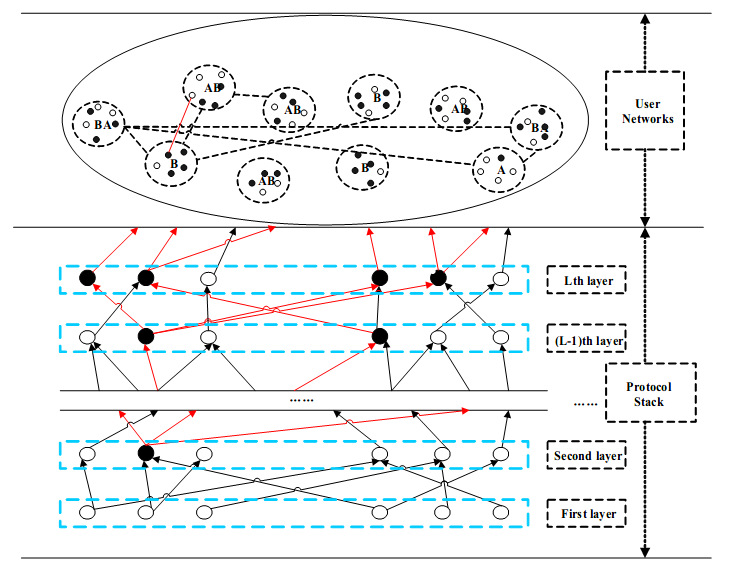
\includegraphics[width=.45\textwidth]{Figure1.png}}
\centerline{Figure 1 Dynamic Evolution Model of Network Protocols}

\subsection{Self-evolution Model}
The Internet protocol stack has a layered architecture that resembles an hourglass. Akhshabi also propose a model based
on the hourglass-shaped Internet protocol stack to explain how the model relates to protocol stacks and evolving network
architectures.The evolution of layered protocol stacks leads to an Hourglass-Shaped Architecture. That help us understand
the self-evolution of the protocols.

\subsection{User Dynamic Behavior Evolution Model(UDBEM)}

\par
\centerline{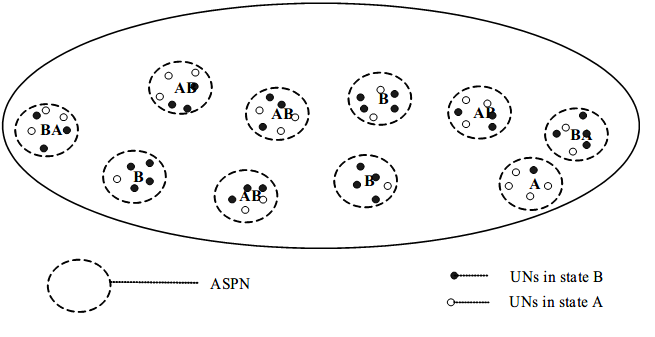
\includegraphics[width=.5\textwidth]{Figure2.png}}
\centerline{Figure 2 Network Topology}

As is shown in Figure 4, there are two kinds of nodes, User Nodes(UN) and Application Service Provider Nodes(ASPN).
The UN is someone who choose the service provided by a new protocol. The UNs are different according the protocols
they chose, for example, the network layer is a network composed of routers and ISP[42]. The ASPNs provide service
for UNs, for example ISP can provide Internet service for users and they can get profits from users. A ASPN can provide
service for dozens of UNs. The UNs can establish a physical topology, while the relationship between UNs and ASPNs form
a logical network. The UNs have two states A and B, where A represents the user still use the current protocol, B states
indicates that the UN choose another new protocol which can provide the same service compared with the old one. The
more B state users, the better adaptability of the new protocol has. The ASPNs have four states, A, B, BA and AB,
where states A represents that the ASPN can only provide the service of protocol A, service B cannot be provided,
vice versa, while states AB indicates the the ASPN can provide the service of protocol A, and compatible conversion
interface for protocol A users of protocol B, vice versa.

The transition strategy between ASPN and UN is as follows:
The transition strategy between ASPN and UN depends on the utility of them, so the utility \(U_{A}\) of a single UN
in state A is:
\begin{displaymath} \label{eq:eps}
U_{A}=\alpha_{A}+\beta Nx_{A}+\beta N(1-q_{A})x_{B}
\end{displaymath}
where \(\alpha\) in (\ref{eq:eps}) represents the utility provided by protocol A, \(Nx_{A}\)indicates the amount of
A users who communicate to this protocol A user and \(\beta Nx_{A}\) represents the whole utility provided
by \(Nx_{A}\)users who communicate to each other. \(\beta\)is the influence coefficient controled by network.
And \(Nx_{B}\)represents the numbers of protocol B user who communicate to this A user and the \(\beta N(1-q_{A})\)
represents the utility provided by \(N_{B}\)protocol B users who choose the BA converter.The \((1-q_{A})\)indicate the
utility comes from A state users interact to the A state users. Similarly understood, the utility \(U_{B}\)of a single UN in
state B is (\ref{eq:eps}):
\begin{displaymath}\label{eq:eps}
U_{B}=\alpha_{B}+\beta Nx_{B}+\beta N(1-q_{B})x_{A}
\end{displaymath}
The utility \(U_{ASPN(A)}\) of the ASPN in state A is (\ref{eq:eps}):
\begin{displaymath}\label{eq:eps}
U_{ASPN(A)}=\alpha_{A}+N_{1}x_{A}+N_{2}x_{B}+N_{3}x_{B}(1-q_{A})
\end{displaymath}
where \(N_{1}x_{A}\), \(N_{2}x_{B}\) represent the number of the users in state A and state B seprately,
\(N_{3}x_{B}(1-q_{A})\) represents utility of the A state user who communicate to the B state users by
BA converters. Similarly understood, the utility \(U_{ASPN(B)}\)of ASPN in state B is (\ref{eq:eps}):
\begin{displaymath} \label{eq:eps}
U_{ASPN{B}}=\alpha_{B}+N_{1}x_{B}+N_{2}x_{A}+N_{3}x_{A}(1-q_{A})
\end{displaymath}
The utility \(U_{ASPN(AB)}\)of the ASPN in state AB:
\begin{displaymath}
U_{ASPN{AB}}=\alpha_{A}+N_{1}x_{A}+N_{2}x_{B}+\sum_{i=0}^{Nx_{B}}(1-q_{B})N_{i}x_{B}
\end{displaymath}
where \(\sum_{i=0}^{Nx_{A}}(1-q_{A})N_{i}x_{B}\) is the utility that \(N_{i}x_{A}\) communicate to the B state users
within ASPN who provided the AB converter, \(N_{i}\) represents the number of B state users who communicate to the ith node.
Similarly understood, the utility \(U_{ASPN(BA)}\) of the ASPN in state BA:
\begin{displaymath}
U_{ASPN(BA)}=\alpha_{B}+N_{1}x_{B}+N_{2}x_{A}+\sum_{i=0}^{Nx_{B}}(1-q_{B})N_{i}x_{A}
\end{displaymath}
Whether the state will change at a time depending on whether the node can obtain more utility after changing the state.
For the UN, if the switch the protocol from A to B, the following conditions must be met:
\begin{displaymath}
U_{A}+S\leq U_{B}
\end{displaymath}
that is the sum of the utility and the cost for the user from state A to state B less then the utility of state B.
For ASPNs, there are four states of transformation, state A to state AB, state AB to state B, state A to B and state B
to state BA, but the conditions must be met:
\begin{equation}
\begin{aligned}
U_{ASPN(A)}+S \leq U_{ASPN(AB)}\\
U_{ASPN(AB)}+S \leq U_{ASPN(B)}\\
U_{ASPN(A)}+S \leq U_{ASPN(B)}\\
U_{ASPN(B)}+S \leq U_{ASPN(BA)}
\end{aligned}
\end{equation}
The following will introduce the model algorithm in detail.

Firstly, check the initial state of each user of the network according to the new protocol, then set the numbers of
ASPN areas and state of ASPNs. The UDBEM is a discrete-time evolution model, There are two following steps for
every evolution process:
\begin{enumerate}
    \item Calculate all the UNs and ASPNs' utility.
    \item Revise the states for each node according to the transmission policy.
\end{enumerate}
Calculate the utility and revise the states according to the policy after the network reaches a steady state.

\subsection{The ANP Model of Evaluation Based on the Network Connection States}

\subsubsection{Build the Communication Topology}
Every node in the network will reaches to the final state within the dynamic evolution model, as is shown in Figure 5,
the number of B state nodes in the final state. The number of B state users is the appearance of the ANP, while the
reason that causes the protocol selecting is the communication efficiency provided by the protocols. So the relationship
between the ANP and the final stage of evolution is that the UNs and ASPNs will establish a topology and communicate
based on the transmission policy and the state pf the users in the final evolution stage.
\par

\centerline{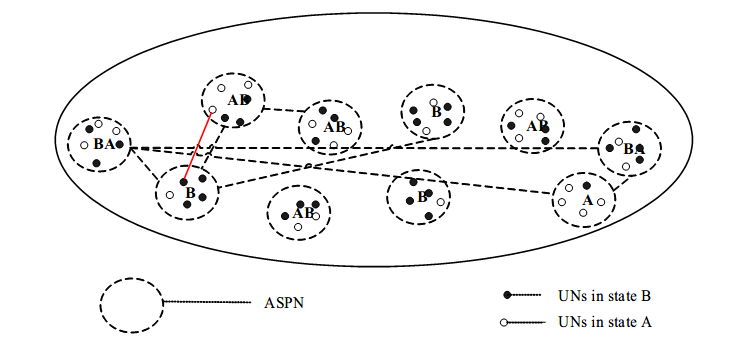
\includegraphics[width=.6\textwidth]{Figure3.png}}
\centerline{Figure 3 The communication network topology }


The connection among the ASPNs is already known to the UNs, and the connection among UNs in different areas charged by
different ASPNs determined by the connection of ASPNs. The connection among the ASPNs is shown Figure 5.1, and the
"\(\surd\)" represents the connection can be established between the converters, the "\(\times\)" not.
\par
\centerline{\includegraphics[width=.7\textwidth]{Table1.png}}
\centerline{Table 5.1 connection relationship of ASPNs}

AS we can see from the chart, the ASPNs in different states can only establish connection between the UNs within the
specific ASPN. We obtain the connection relationship as shown in Table 5.2 according to the connectivity rules.
\par
\centerline{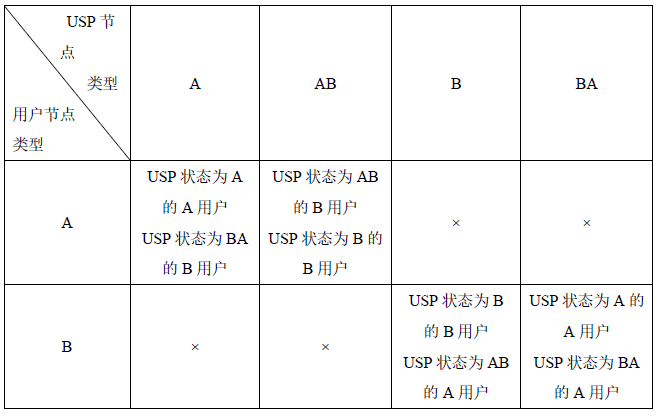
\includegraphics[width=.5\textwidth]{Table2.png}}
\centerline{Table 5.2 connection relationship of UNs}

\subsubsection{Calculate the efficiency of communication}
Assume a communication network topology is a graph $G$ which has $M$ edges, $N$ points, so the communication efficiency
is calculated as follows:
\begin{enumerate}
    \item Firstly,  according to the position and the state of the nodes, we can establish a cost function \(F(i,j)=\eta (\eta \ge1)\)
    between two nodes, so the communication efficiency of each edge \(e_{i,j}\) is \(1/\eta\).
    \item Then, the communication efficiency between $i$,$j$ is \(\varepsilon_{i,j}\), which can be expressed as the
    sum of every edge communication efficiency
    \begin{displaymath}
    \varepsilon_{i,j}=\sum\frac{1}{F(i,k)}+\frac{1}{F(k,r)}+\cdots+\frac{1}{F(s,j)}
    \end{displaymath}
    where $k$, $r$...$s$ are the shortest path sequences which pass the $i$,$j$.
    \item The communication efficiency of $G$ is $E(G)$
    \begin{displaymath}
    E(G)=\sum_{i\ne j\notin G}\varepsilon_{ij}/[N(N-1)]
    \end{displaymath}
    as you can see, the more close to 1 of $E(G)$, the closer the value of $E(G)$ is to 1, the higher the communication efficiency.
    We can get the indicators of the ANP by calculated the $E(G)$, then evaluate the ANP.
\end{enumerate}

\section{Model Analysis}
\subsection{Self-evolution}
\par
\centerline{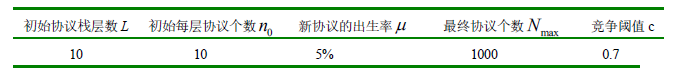
\includegraphics[width=.7\textwidth]{Table3.png}}
\centerline{Table 3.1 Basic Parameters}
As is shown in Figure 3.8, 3.9 and 3.10, the new protocol layer in the protocol stack 10, 50, 100, its initial proportion
of the new protocol is the first after decreasing increasing trend. So the initial proportion is minimum of intermediate
layer, while from the middle to upper or lower layer showing an increasing trend initial proportion. The protocols in the
middle layer is hard to survive and has a small proportion if the protocols are deployed in the network. The reason for
this phenomenon is the protocol stack presented hourglass, the lower and higher layers tend to have more survival and the
waist of the hourglass appear has less survival.

\subsection{Evolution Model Based on Dynamic Section of User Behavior}
The basic parameters of the experiment described as shown in Table 4.1,
\par
\centerline{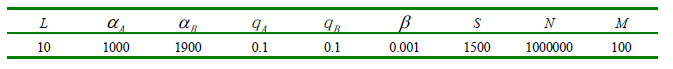
\includegraphics[width=.7\textwidth]{Table4.png}}
\centerline{Table 4.1 Basic parameters}

\subsubsection{The Influence of the Protocol Utility to Adaptability}
As is shown in Figure 4.1, the ANP will increase if we increase the utility of protocol B, we can get the penetration
changes with time of protocol B with the different $\alpha_{B}/\alpha_{A}$. The higher utility of a new protocol, the
less time needed to get the whole penetration. You can see the penetration varying depending on the different
$\alpha_{B}/\alpha_{A}$ in Figure 4.4. When the new protocol provides for its own utility 1.8 times the current, the
case of penetration of the new protocol dose not change. The reason is that the current utility is greater than the
new protocol under the current network state. When the new protocol provides for its own utility is 1.8 times of the
current and the simulation proceeds to the 50th,  the new protocol get 100 percent penetration, which entirely depends
on the parameters of the experiments selected. When the new protocol provides for its own utility is 4 times of the
current and the simulation proceeds to the 10th, the new protocol get 100 percent penetration.

\subsubsection{The Influence of the External Network Utility to the Adaptability}
As is shown in Figure 4.5, the ANP will increase if we increase the network utility. When the utility of the external
network value is too large, it will hinder the new protocol to enhance the proportion. The picture shows the changes
in the penetration of the new protocol under different utilitise of the external network effect \(\beta\). The value of
$\alpha_{B}/\alpha_{A}$ is fixed at 1.9 to ensure that the new protocol is acceptable to the user. When there is no
external network utility, that is $\beta=0$, the penetration of the new protocol stops at 67.4\%. As the new protocol
of its own utility, so the state A users are willing to switch to state B to obtain higher returns, Some A-State users
have already achieved high utility in the existing network environment, and the transition to state B does not get higher
utility, so the user chooses to keep the existing state, which is why the new protocol's penetration rate will stop.
An increase in the external utility from the state B user increases the number of users switching to the B state, which
encourages the user to switch to the state B. When $\beta$ is 0.001, the new protocol can be completely infiltrated. If
the external network utility is too large, will inhibit the penetration of the new protocol.For example, when $\beta$ is
0.010, since the state A user occupies a considerable proportion of the initial state and get enough income, so the state
users do not need to convert the state to obtain additional utility, so the new protocol Of the penetration does not
change. If we set the new protocol can reverse the conversion, B protocol users will choose to switch to B state to get
more utility. At this point the utility of excessive external network will not only promote the penetration of the new
protocols but will inhibit the adaptability of them.

Figure 4.1
\subsubsection{The Influence of the Converter to the Adaptability}
The result of simulation indicates that, the increasing utility of AB converter []. As expected, the efficient AB
converter can reduce the cost of state transition A to B. However, the efficient converter AB can bring utility of
B to A from the perspective of individual, so there is not any incentive for A with or without converter BA.

From the other hand, after the users changing the state A to B encouraged by BA converter, they can get the utility
from other state A users and  B state users changed from state A. As is shown in the simulation results, at most cases,
the ANP will improve if the utility of BA converter increase. The Figure 4.6 indicates that, when the efficiency of
the BA converter is 92.5\%, it will take more time for the new protocol to get to the full penetration than the
efficiency of the converter is 98\%. Besides, we draw the conclusion that penetration can be blocked when we improve
the efficiency of the converter in some case. When BA converter efficiency from 92.5\% to 94.5\%,  the penetration
of the new protocol will stop at 95\%. The reason is when the simulation is stopped, the A state users will get more
utility than cost for changing to state B. For the remaining A state users, since more and more users change to state B,
they will get more utility from B state users. Efficient BA converter will increase the utility generated by state B
users, so more users will be encouraged to state B. Since the BA converter is bidirectional, efficient BA converter
will increase the utility for remaining A state users and preventing them from converting to state B.The result suggests
that the ANP will improve if we increase the efficiency of the converter BA and keep a low level. Furthermore, the
efficiency of the BA converter must be maintained at a certain range in order to promote the new protocol fully penetrate.

Figure 4.6
\subsection{Evaluation Model of the ANP Based on Network Connection Status}
There 10 million nodes in the network topology, we take the cost of the connection between two nodes is $varepsilon=4$ ,
so the communication efficiency $1/\varepsilon$ is 0.25 of any edge $e_{i,j}$.
\subsubsection{The Influence on Communication Efficiency  of the Protocol Utility}
Figure 5.2 shows the changes of the communication efficiency at different $\alpha_B/\alpha_A$,when $\beta=0.001$. As is
shown in the picture, the communication efficiency of the network grows faster and has significantly improved with the
development of the utility of the new protocols. It can be concluded that improving the efficiency of the new protocols
will help to improve the communication efficiency of the network, that is, improving the efficiency of the new protocols
will help to improve the ANP.

Figure 5.2
\subsubsection{The Influence on Communication Efficiency of the External Network Utility}
Figure 5.3 shows the changes of the communication efficiency at different $\beta$ and $\alpha_{B}/\alpha_{A}=1.5$. As is
shown in the picture, the communication efficiency has improved with the improvement of the external utility of the network.
But when the utility reaches to a certain value, the communication efficiency of the network significantly reduced. It
can be conclude that improving the external network utility will help to improve the communication efficiency, but the
efficiency will decrease when the external network utility is to high. So improving the external network utility
appropriately helps to improve the ANP of new protocols.

Figure 5.3
\subsubsection{The Influence on Communication Efficiency of Converters}

Figure 5.4
Figure 5.4 shows the changes of the communication efficiency while $\beta= 0.001$, $\alpha_B/\alpha_A=1.5$, at different
conversion efficiency of the BA converter. As is shown in the picture using converter can improve the communication efficiency,
but the communication efficiency of the network will decrease when the utility of BA converter grows to a certain range.
While if the efficiency if the converter is high enough, it dose greatly improve the communication efficiency of the network.
It can be concluded that improving the efficiency of the converters appropriately helps to improve the ANP.

\section{Simulation Analysis}
\subsection{Comparative Experiments A and B}
The basic experiment parameters are set as follows,
\par
\centerline{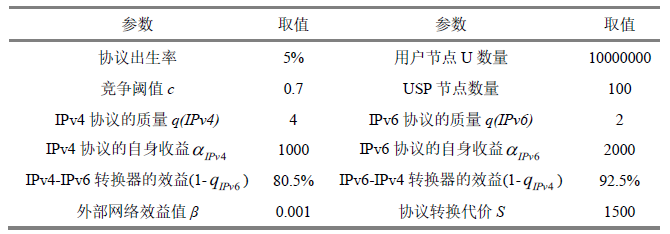
\includegraphics[width=.7\textwidth]{Table5.png}}
\centerline{Table 6.1 Basic Parameters}
The Figure 6.2 represents the average probability of IPv4 and IPv6 exist in the stack after modeling the self-evolution
many times. As we can see from the result, the more the number of experiments, the probability of the final IPv6 protocol
decreases in the protocol stack. It can be seen in the evolution of the protocol stack that the IPv4 protocol cannot be
fully replaced by the IPv6. The reason is that, the greatest contribution of IPv6 is to provide more addresses not
additional new services compared to IPv4. The upper layer service of IPv4 and IPv6 is almost no difference,  so there
is competition between IPv4 and IPv6 protocol. IPv6 protocol is not widely deployed, so its quality indicators is lower
than IPv4, that's why IPv4 is more competitive than IPv6. Much work need to be done if want replace the IPv4 by IPv6
protocol. On the one hand, IPv6 should provide some services that cannot provided by IPv4, which means that IP has more
service nodes in the upper layer than IPv4. On the other hand, the competition should be avoided between IPv4 and IPv6,
particularly in the deployment of the IPv4 is much higher than IPv6 protocol. Under these circumstances, we can make
IPv6 as a "Second layer protocol" to provide services for the upper layer not a competitive protocol to IPv4.

Table 6.3, 6.4

As is shown in Figure 6.3, when the utility of external network $\beta=0.001$, the efficiency of IPv6-IPv4 converter is 
92.4\% and the IPv4 and IPv6 protocol utility ratio $\alpha_B/alpha_A$ is 2, the IPv6 can be accepted and completely 
replace IPv4 to achieve the full penetration, although it develops slowly.   The reason is that the government promote 
the deployment of IPv6 vigorously which can make up for the economic losses during the deployment. If the adaptability 
of the IPv6 wanted to be improved, we can do it in three ways: improve the utility of IPv6 protocol, to make it more 
competitive compared to IPv4; Improve the external utility of the protocol, the government can make up for the economic 
losses for deploying the IPv6 protocol; Improve the efficiency of IPv6-IPv4 converter, let the IPv4 users are willing 
to use the IPv6 protocol.

\subsection{The comparative Experiments of UDP and DCCP}
The basic experiment parameters are set as follows,
\par
\centerline{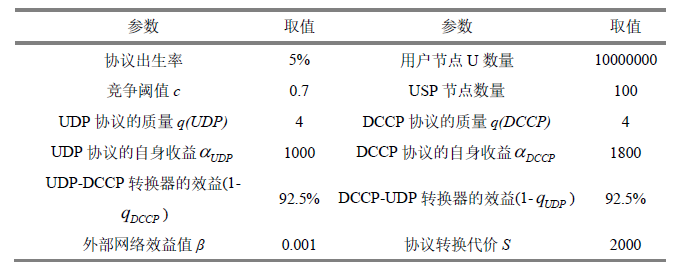
\includegraphics[width=.6\textwidth]{Table6.png}}
\centerline{Table 6.2 Basic Parameters}
The Figure 6.4 represents the average probability of UDP and DCCP exist in the stack after modeling the self-evolution 
many times. As we can see from the result, the more the number of experiments, the probability of the final DCCP 
protocol decreases in the protocol stack.  It can be seen in the evolution of the protocol stack that the UDP protocol 
cannot be fully replaced by the DCCP.

Figure 6.5 6.6

We build 7860000 UDP users and 2140000 DCCP users in the network which has 10000000 nodes, utilizing the UDP users 
share and DCCP users share from the protocol self-evolution model and according to the evolution model based on 
dynamic selection of user behavior. All the users reached to steady state after a period of evolution. As is shown 
in Figure 6.5,when the utility of external network $\beta=0.001$, the efficiency of DCCP-UDP converter is 92.4\% 
and the IPv4 and IPv6 protocol utility ratio $\alpha_B/\alpha_A$ is 1.8, the DCCP can be accepted and completely 
replace UDP to achieve the full penetration, although it develops slowly. Besides, when the DCCP share reaches around 
39\%, it will not change any more. If the adaptability of the DCCP wanted to be improved, we can do it in three ways: 
improve the utility of DCCP protocol, to make it more competitive compared to UDP; Improve the external utility of 
the protocol, the government can make up for the economic losses for deploying the DCCP protocol; Improve the efficiency 
of DCCP-UDP converter, let the UDP users are willing to use the DCCP protocol.
\section{Conclusion}
We can draw some conclusions from the protocol self-evolution simulation. First,  the protocols at the waist of 
the hourglass appear to have less survival, while the lower and higher layers tend to live longer and easier. 
Second, if we improve the utility of the protocol, the external utility of the protocol and the efficiency of 
the converters appropriately can play important roles in improving the ANP. Third, the higher efficiency of the 
communication, the better ANP by establishing network topology based on the interact policy of the users and 
nodes. Forth and last, the network protocol adaptability evolution model we proposed can be applied to assess 
the ANP, according to the comparative experiments of IPv4, IPv6 and UDP and DCCP. The network protocol adaptability 
evolution model guiding significance for the development and deployment of the network protocols.

Our model can simulate the dynamic evolution of the new protocols, furthermore, to measure the adaptability 
through the communication efficiency of the network topology established. In addition to this, we also proposed 
methods to improve the ANP. But we still have some shortcomings about the model need to be further refined and 
improved. In the future, we can establish a protocol dynamic evolution model and check by simulating,  then 
evaluate the ANP by deploying to the real networks. We can also focuse on other factors which affect on the 
ANP, increase the availability of the model.
\end{document}
